\documentclass[class=article, crop=true]{standalone}
\usepackage{tikz}
\usepackage{subcaption}
\usepackage[subpreambles=true]{standalone}
\begin{document}

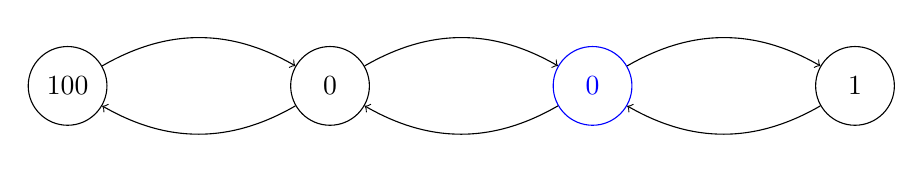
\begin{tikzpicture}
\node (A) at (-5, 0) [minimum size=1cm, circle, draw, color=black] {$100$};
\node (B) at (-1.667, 0) [minimum size=1cm, circle, draw, color=black] {$0$};
\node (C) at (1.667, 0) [minimum size=1cm, circle, draw, color=blue] {$0$};
\node (D) at (5, 0) [minimum size=1cm, circle, draw, color=black] {$1$};
    
\draw (A) edge [bend left, ->] (B);
\draw (B) edge [bend left, ->] (C);
\draw (C) edge [bend left, ->] (D);
    
\draw (D) edge [bend left, ->] (C);
\draw (C) edge [bend left, ->] (B);
\draw (B) edge [bend left, ->] (A);
\end{tikzpicture}

\end{document}